\documentclass[tikz,border=5pt]{standalone}
\usetikzlibrary{calc}

\begin{document}
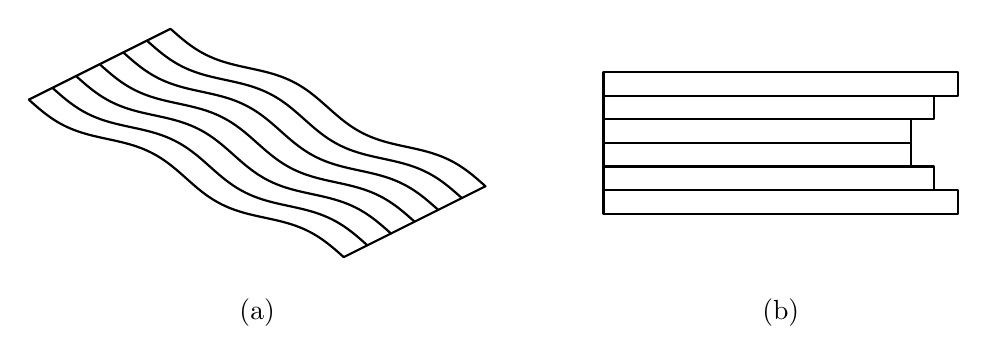
\begin{tikzpicture}[line join=round, line cap=round]

	% ==========================================
	% FIGURE (a): Wavy Parallelogram
	% ==========================================
	\begin{scope}[local bounding box=figA]
		\coordinate (A) at (0, 0);
		\coordinate (B) at (-4, 2);
		\coordinate (C) at (-5.8, 1.1);
		\coordinate (D) at (-1.8, -0.9);

		% Straight side caps
		\draw[thick] (A) -- (D);
		\draw[thick] (B) -- (C);

		% Draw 7 wavy lines (6 strips)
		\foreach \i in {0,...,6}{
				\pgfmathsetmacro{\t}{\i/6}
				\draw[thick, samples=100, domain=0:1]
				plot (
					{ (1-\x)*(0*(1-\t) + -1.8*\t) + \x*(-4*(1-\t) + -5.8*\t) + 0.05*sin(\x*360*2) },
					{ (1-\x)*(0*(1-\t) + -0.9*\t) + \x*(2*(1-\t) + 1.1*\t) + 0.08*sin(\x*360*2) }
				);
			}
	\end{scope}

	% ==========================================
	% FIGURE (b): 6 Stepped Rectangular Bars
	% ==========================================
	% Placed relative to figA's vertical center line
	\begin{scope}[xshift=1.5cm, yshift=0.55cm, local bounding box=figB]
		\pgfmathsetmacro{\h}{0.3} % Height of each bar
		\pgfmathsetmacro{\totalH}{6 * \h} % Total height = 1.8cm

		% Draw 6 stacked bars centered vertically around y = 0
		\foreach \i/\len in {0/4.5, 1/4.2, 2/3.9, 3/3.9, 4/4.2, 5/4.5}{
				\draw[thick]
				(0, \i*\h - \totalH/2) rectangle (\len, \i*\h + \h - \totalH/2);
			}
	\end{scope}

	% ==========================================
	% LABELS (Aligned horizontally at fixed Y)
	% ==========================================
	\coordinate (L) at (0, -1.6); % Shared bottom baseline level

	\node at (figA.center |- L) {(a)};
	\node at (figB.center |- L) {(b)};

\end{tikzpicture}
\end{document}
